\section{Results}
\label{sec:results}

In this section, ...


\subsection{Overall Overview}
\label{qual_res}

Our initial aim was to capture a snapshot of the current developments of the entertainment and gaming industry, including its potential future trajectory. However, we also undertook a supplementary collection of health-related devices. We decided on this as even though our search term was not intended to find papers concerning health-related devices, the IEEExplore Library still provided papers in that field of research. This was considered as reasonable as it would also allow as to draw connections of possible evolutions of 3D interfaces from the healthcare sector into the entertainment sector.

However, we did not evaluate the health-related devices in detail only included them in our broad categorization, seen in Figure~\ref{fig:broad}. A few reasons for this decision:

Health-related devices are designed for specialized tasks. Their functionalities and implications are vast, often requiring a detailed, domain-specific understanding which differed from our primary sectors of focus.

While one of our sub goals was to forecast future trends, the sheer breadth and depth of the health domain hinted at a vast potential that would be best addressed in a dedicated study.

Given these considerations, we believed it was in the best interest of the study's clarity and precision to focus on the domains outlined by our original search term: Gaming and Entertainment. 


\subsection{Broad Categorization}
\label{ss: broad}
As mentioned we used the taxonomy by Adilkhanov et al.~\cite{Adilkhanov22} to get a first broad categorization of the devices we found during our literature review. In Figure~\ref{fig:broad} the entries on the left in black are the categories developed by the other paper. We added some new categories, as we could not put every device we found into the existing categories. Therefore, we extend the taxonomy by adding the categories: "Camera", "Foot-worn" and "Skin-attached". Furthermore, we divided the devices into the categories: Gaming, Health, Music and Entertainment. 

Now we discuss, the categories in more detail. Grounded haptic devices are typically too large or complex to be worn on the user's body. They often have limited workspace due to their stationary nature. Grounded haptic systems can be further categorized into graspable and touchable devices. 

Graspable haptic devices are primarily kinesthetic and are known for their precision and ability to provide a wide range of forces. They are designed to mimic the sensation of grasping or manipulating physical objects in a virtual environment. 

Touchable haptic devices are interactive displays that allow users to tactilely interact with objects shown on the screen. They typically offer pure cutaneous feedback through various actuation methods, making them suitable for applications like user interfaces and entertainment.

Camera-based devices use visual sensors and tracking technologies to capture and interpret the user's movements or gestures. These devices are used for applications such as gesture recognition, augmented reality, and 3D modeling. 


Hand-held haptic devices can be picked up and held by the user without the need for body attachment. They are generally lighter and offer a larger workspace than grounded devices. They can provide both kinesthetic and tactile feedback. 


Direct actuation hand-held devices operate directly on the user's hand through the handle and end-effector, providing haptic feedback through mechanisms. 

Indirect actuation hand-held devices change the centre of gravity to deliver different haptic cues, allowing for the simulation of various virtual tools without requiring separate proxy objects. 

Wearable haptic devices are designed to be worn on the user's body. They can provide various forms of haptic feedback, such as kinesthetic and cutaneous sensations. 

Head-worn devices are haptic devices that are worn on the user's head, typically in the form of headsets. They are commonly used in virtual reality and augmented reality applications, providing immersive experiences.
 
Body-worn haptic devices are designed to be worn on different parts of the user's body other than the head. These devices can provide haptic feedback to specific body regions, enhancing the overall immersive experience.

Finger-worn haptic devices, often referred to as thimbles, focus on providing tactile stimulation to the fingerpads. They are particularly suitable for fine control and manipulation tasks involving the fingertips. 

Arm-worn haptic devices are designed to be worn on the user's arms. They can provide haptic feedback to the arms and are used in applications that require simulating arm-related interactions. 

Foot-worn haptic devices are worn on the user's feet and are used for simulating interactions related to the feet or lower limbs. They find applications in virtual environments involving walking or foot-based tasks. 

Skin-attached haptic devices are directly attached to the user's skin, providing cutaneous feedback. These devices are often used for applications requiring precise, localized tactile sensations, such as medical training or virtual surgery simulations.


\begin{figure}[htbp]
	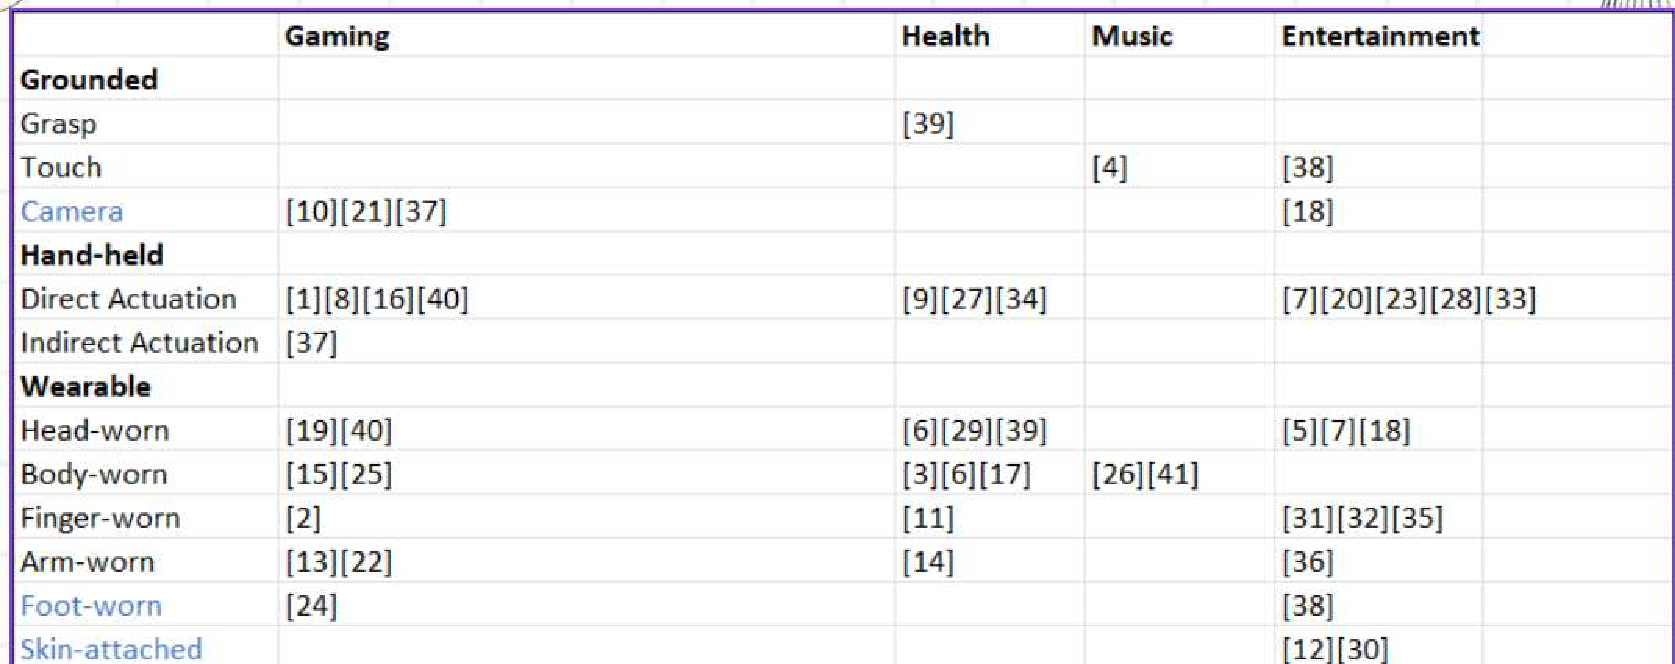
\includegraphics[width=\columnwidth]{figures/broad.pdf}
	\label{fig:broad}
\end{figure}


\subsection{Devices in Music}
The music category only consists of three entries. One of them is a Audino Foot Board used to enhance the experience while learning a new instrument [4]. While the other [26] and [41] used a device called Hapbeat...


\subsection{Devices in Gaming}
\label{gaming}
In the explanation and chart for the gaming landscape we have looked at 3D interfaces, especially as they address to virtual and mixed reality. To get a more detailed categorization we used the papers from our literature review to start a bottom-up categorization approach. However, as we knew from the categorization seen in Figure~\ref{fig:broad}, we already settled on our categories which will be on top. Through a detailed bottom-up approach we have categorized these interfaces based on which body part used the device. To give a rough understanding of how that process looked like we do one example step-by-step. In [21] there is a camera used to do... . Therefore, we added the category "Camera". We repeated this process for each paper. Then we looked at similar devices. Therefore, we added "Sensor" [10] and "Camera" into the category of "Visual", which means that these device represent what they capture in a visual way. Due to this, we had to categorize "Touch" and "Grasp" into the "Contact" category, as these devices need some form of human touch to work. Both of these categories where eventually connected to the "Grounded" categories as we placed the devices before the subcategorization in that.


\begin{figure}[htbp]
	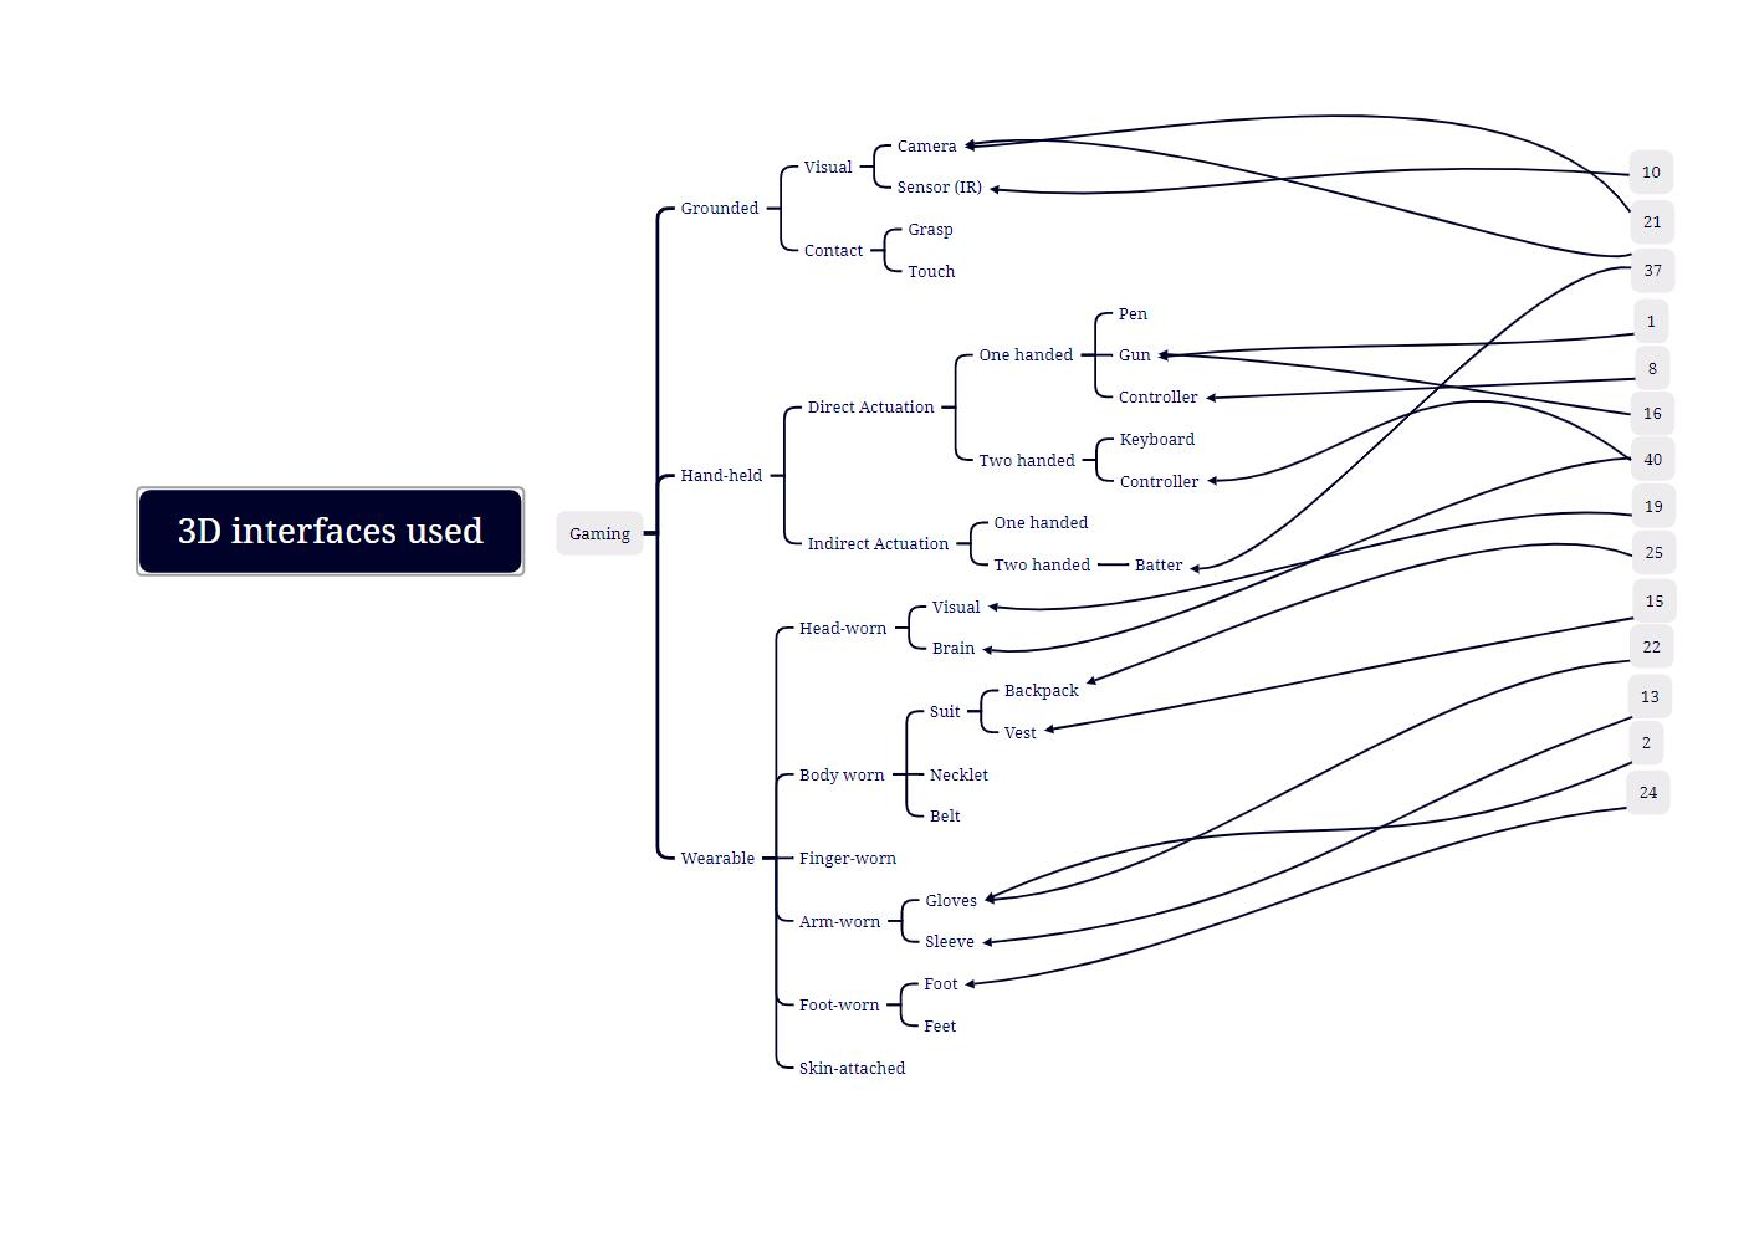
\includegraphics[width=\columnwidth]{figures/gaming.pdf}
	\label{fig:gaming}
\end{figure}
 

In the following, we only present some of the devices developed in the last 5 years. 
VR treadmill system (leap motion) coupled with a handheld 3D interface. The device is meant to be used for whole body and detect a leap when necessary. Gaming has added a new perspective on jumping over objects and it's a key movement on games these days. The sensors work simultaneously so the axis also can be changed with a little offset as well.

The design and implementation of a VR gun controller with haptic feedback. The gun(s) have a feedback motor and when attached to a real print of the gun added to visual devices will give the user experience like being in a real situation. Without the feedback it would feel more poor and have a lack of sensation. The motor it's self is quite simple creation but the way they have included it in a bigger entity makes it create a whole new level to the gaming.

Wack-a-mole styled hammer for games. The tool itself has a sensors, but it's also being tracked by cameras that have been grounded next to the system. The user can either see the gameplay happening on screen or by using a visual headset (VR). The second will create a more live-like experience due the high precision for it.

\subsection{Devices in Entertainment}
\label{entertainment}

\begin{figure}[htbp]
	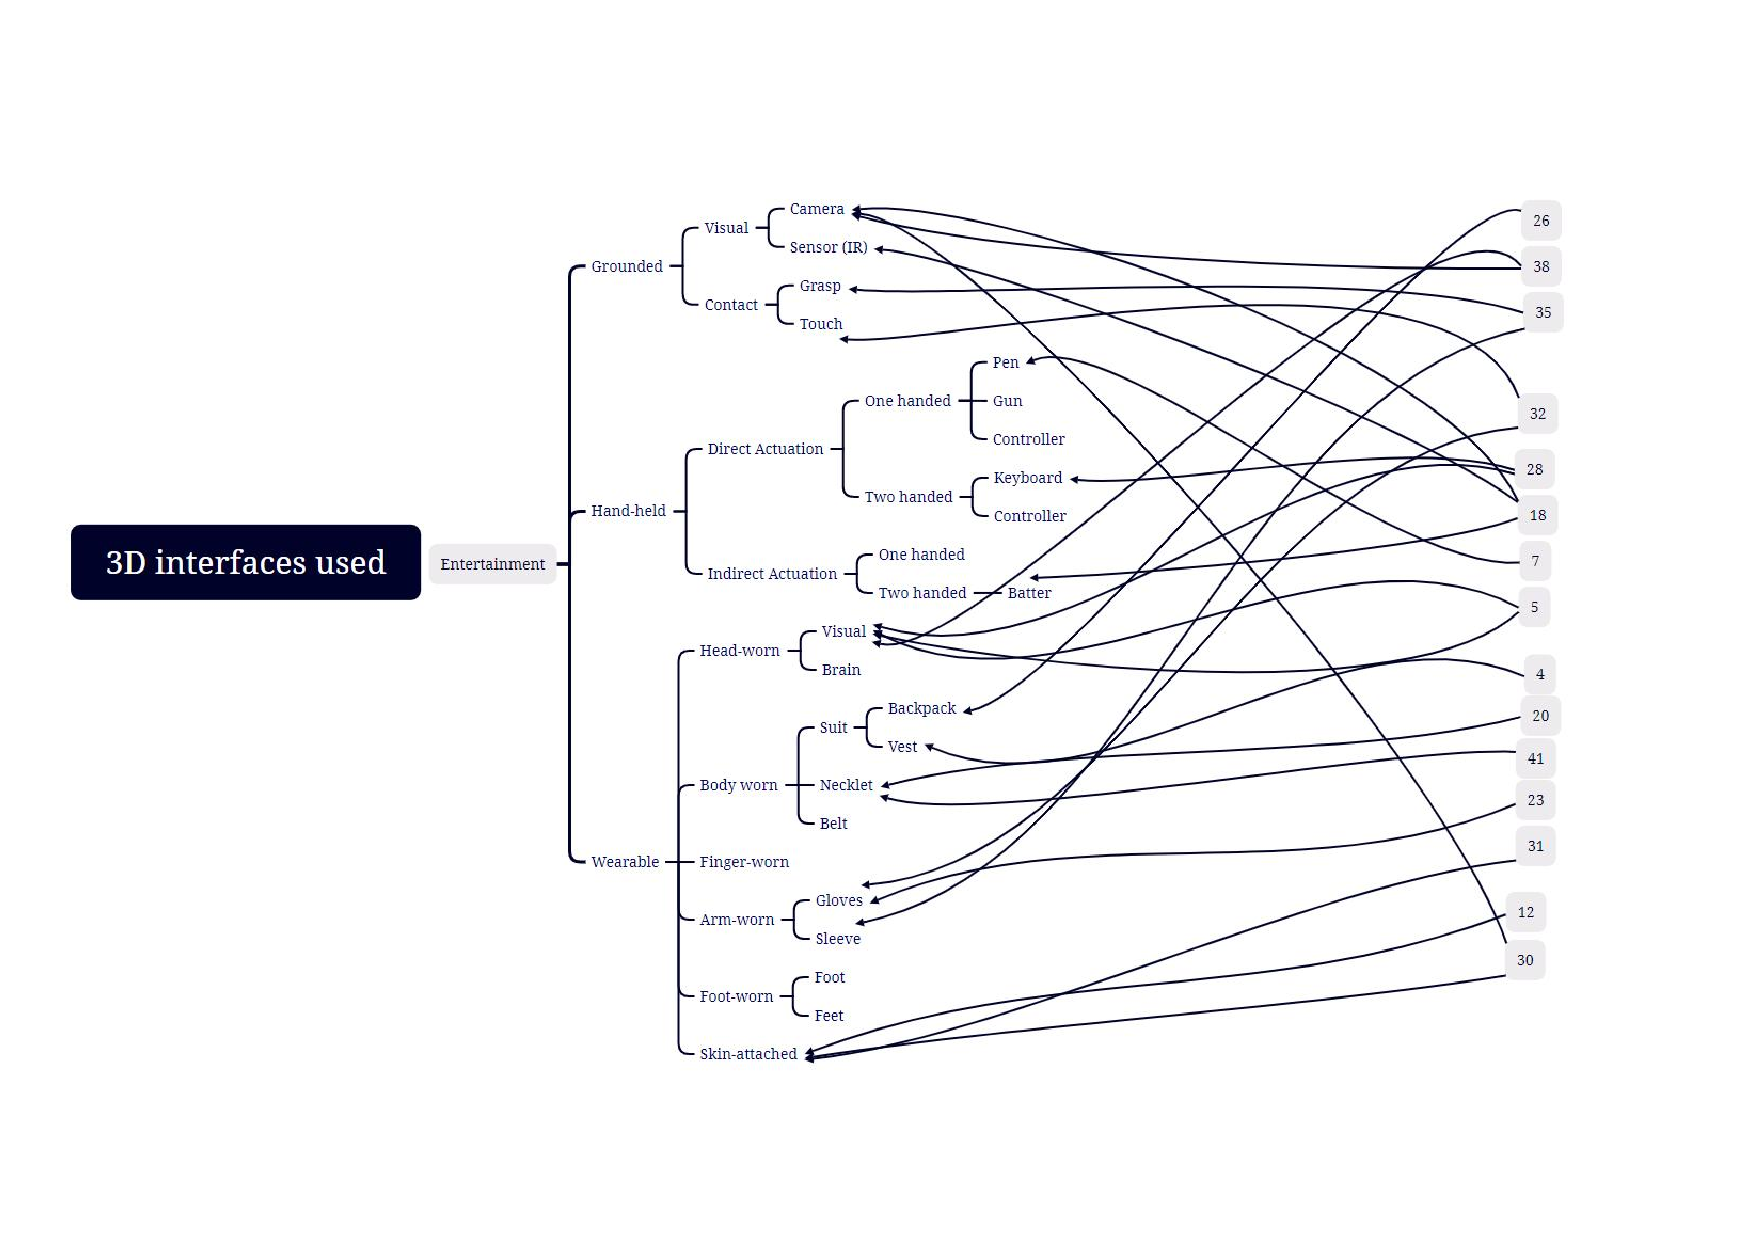
\includegraphics[width=\columnwidth]{figures/entertainment.pdf}
	\label{fig:entertainment}
\end{figure}


Haptic sensors for feet, can be used to define the motion of and placement. The sensors are meant to be used with two feet at the time but they also can be used individually for different kind of tasks. 

A high-fidelity and high-precision multi-surface pen for virtual reality. With the pen the drawing does not only happen in a 2D space like we have been used to, it can also create objects and multiple different lines in 3D space making the visual outcome a lot of different compared to the normal pen that we are used to.

Soft microtubule muscle-driven 3-axis skin-stretch haptic device. The device tracks basically movement on a very high accuracy, so completing tasks with fingers like some different grips are made to be more normal and the feedback feels more like real life.



\subsection{The Importance of Subcategorization}

The importance of subcategories becomes evident when examining user interactions. While broad categories provide an overview of interface options, the subcategories offer tailored solutions that cater to individual needs. For example, within the realm of hand-held interfaces, choices extend beyond general preferences. Some users may favor a one-handed controller due to its ergonomic design, which can minimize arm strain and align better with natural postures. Others might gravitate towards a two-handed controller, valuing its stability and comprehensive button layout. By diving into these specific nuances, we can design interfaces that not only meet functional requirements but also prioritize user comfort and intuitive use. This meticulous attention to detail ensures enhanced usability and heightened user satisfaction. 

Furthermore, the Figures~\ref{gaming}\ref{entertainment} show that there is no commonly settled device being developed in research. None of the subcategories in the gaming sphere contain more than two devices. This may indicate that there is still more room for growth as it seems that there is no optimal solution being found. This might also be caused by the fact that devices are individually created for a certain task. Therefore, there is no distinct pattern to see which devices are most commonly used in gaming or entertainment.